\documentclass{beamer}
\usepackage[normalem]{ulem}
\usepackage{hyperref}
\usepackage{tikz}
\title{Mining counterexamples for wide-signature algebras with an Isabelle server}
\author{Wesley Fussner, Boris Shminke}
\institute{Laboratoire J.A. Dieudonn\'e, CNRS, and Universit\'e C\^ote d'Azur, France}
\date{6 Sep 2021}

%\usetheme{lucid}
\begin{document}
\begin{frame}
  \titlepage
\end{frame}
\begin{frame}
  \frametitle{What is a residuated binar}
Binar (magma, groupoid) --- a set with a binary operation $\cdot$

For residuation we add a lattice structure:
\begin{align*}
x\wedge y = y\wedge x \\
x\wedge\left(y\wedge z\right) = \left(x\wedge y\right)\wedge z \\
x\vee y = y\vee x \\
x\vee\left(y\vee z\right) = \left(x\vee y\right)\vee z \\
x\wedge\left(x\vee y\right) = x \\
x\vee\left(x\wedge y\right) = x
\end{align*}
\end{frame}
\begin{frame}
\frametitle{What is a residuated binar (RB)}
A binar with a lattice stucture ($x\le y\Longleftrightarrow x=x\wedge y$) and two residuation operations:

\begin{align*}
  x\cdot y\le z\Longleftrightarrow x\le z/y\Longleftrightarrow y\le x\backslash z
\end{align*}  
\end{frame}
\begin{frame}
  \frametitle{Some distributive laws hold in all RBs}
\begin{align*}  
x\cdot(y\vee z)= x\cdot y\vee x \cdot z\\
(x\vee y)\cdot z= x\cdot z\vee y\cdot z \\
x\backslash (y\wedge z) = x\backslash y\wedge x\backslash z \\
(x\wedge y)/ z = x/ z\wedge y/ z \\
x/ (y\vee z) = x/ y\wedge x/ z \\
(x\vee y)\backslash z = x\backslash z\wedge y\backslash z
\end{align*}
\end{frame}
\begin{frame}
  \frametitle{And some don't (in general)}
\begin{align*}  
x\cdot(y\wedge z)= x\cdot y\wedge x\cdot z \\
(x\wedge y)\cdot z= x\cdot z\wedge y\cdot z \\
x\backslash (y\vee z) = x\backslash y\vee x\backslash z \\
(x\vee y)/ z = x/ z\vee y/ z \\
(x\wedge y)\backslash z = x\backslash z\vee y\backslash z \\
x/ (y\wedge z) = x/ y \vee x/ z
\end{align*}
\end{frame}
\begin{frame}
But some distributivity laws can
\begin{itemize}  
\item follow from a combination of others
\item under special circumstances
\item \href{https://doi.org/10.1007/s00012-019-0625-1}{Fussner, W., Jipsen, P. Distributive laws in residuated binars. Algebra Univers. 80, 54 (2019)}
\end{itemize}
\end{frame}
\begin{frame}
\frametitle{Example from cited paper}
If $(x\wedge y)\vee z = (x\wedge z)\vee (y\wedge z)$ (distributive lattice) then:
\begin{align*}
(x\vee y)/ z = x/ z\vee y/ z \\
(x\wedge y)\backslash z = x\backslash z\vee y\backslash z \\
\Longrightarrow x\backslash (y\vee z) = x\backslash y\vee x\backslash z
\end{align*}
\end{frame}
\begin{frame}
\frametitle{Non-example}
If $(x\wedge y)\vee z = (x\wedge z)\vee (y\wedge z)$ then there is a counter-example for:
\begin{align*}
x\cdot(y\wedge z)= x\cdot y\wedge x\cdot z \\
(x\wedge y)\cdot z= x\cdot z\wedge y\cdot z \\
\Longrightarrow x\backslash (y\vee z) = x\backslash y\vee x\backslash z
\end{align*}
\end{frame}
\begin{frame}
\frametitle{Open Problem}
In a residuated binar which of the following distributivity laws follows from some combination of others:
\begin{align}
\label{eqn:1}  
x\cdot(y\wedge z)= x\cdot y\wedge x\cdot z \\
\label{eqn:2}  
(x\wedge y)\cdot z= x\cdot z\wedge y\cdot z \\
\label{eqn:3}  
x\backslash (y\vee z) = x\backslash y\vee x\backslash z \\
\label{eqn:4}  
(x\vee y)/ z = x/ z\vee y/ z \\
\label{eqn:5}  
(x\wedge y)\backslash z = x\backslash z\vee y\backslash z \\
\label{eqn:6}  
x/ (y\wedge z) = x/ y \vee x/ z
\end{align}
\end{frame}
\begin{frame}
\frametitle{Problem}
\begin{itemize}
\item 6 non-trivial distributivity laws
\item $(2^5 - 1) \times 6$ of possible implications between them
\item adding: $\cdot$ commutativity/associativity, lattice modularity, involution operation, ...
\item often a counter-examples exists
\end{itemize}
\end{frame}
\begin{frame}
\frametitle{Why so many?}
\begin{itemize}
\item if \ref{eqn:1},\ref{eqn:2},\ref{eqn:3},\ref{eqn:4},\ref{eqn:5} doesn not imply \ref{eqn:6}
\item then neither \ref{eqn:1},\ref{eqn:2},\ref{eqn:3},\ref{eqn:4} implies \ref{eqn:6}
\item but we don't know what is true in the beginning
\item finding counter-examples for more general statements is harder  
\end{itemize}
\end{frame}
\begin{frame}
\frametitle{Task}
\begin{itemize}
\item thousands of hypotheses
\item counter-examples structure is important for understanding
\item we want to check as many hypotheses as possible
\item starting with the least general ones  
\end{itemize}
\end{frame}
\begin{frame}
\frametitle{How to find provable hypotheses?}
\begin{itemize}
\item encode the hypothsis into some formal language
\item give it to one's favourite counter-examples finder:
\item Mace4, Paradox, Kodkod, ...  
\item wait for a couple of minutes and repeat
\end{itemize}
\end{frame}
\begin{frame}
\frametitle{How to find provable hypotheses?}
\begin{itemize}
\item \sout{give it to one's favourite counter-examples finder} which one?
\item \sout{wait for a couple of minutes} why hours or days?
\item \sout{repeat} but we have thousands of candidates to check
\end{itemize}
\end{frame}
\begin{frame}
\frametitle{How to find provable hypotheses: Isabelle Platform}
\begin{itemize}
\item uses a relatively simple \href{https://github.com/inpefess/residuated-binars/blob/master/involution/task10/T88.thy}{language} for encoding theories
\item provides an interface (through Kodkod) to SMT solvers
\item Isabelle server runs solving tasks \emph{in parallel}
\end{itemize}
\end{frame}
\begin{frame}
\frametitle{Isabelle}
\begin{itemize}
\item is overall great but
\item is written in StandardML and Scala (I used Python for generating theory files)
\item it's server has only TCP API (not even HTTP!)
\end{itemize}
\end{frame}
\begin{frame}
\frametitle{Solution}
\begin{itemize}
\item write a \href{https://github.com/inpefess/isabelle-client}{Python client to Isabelle server}
\item write \href{https://github.com/inpefess/residuated-binars}{scrips for generating and processing} Isabelle theory files
\item parse Isabelle server \href{https://github.com/inpefess/residuated-binars/blob/master/involution/task10/isabelle.out}{log} to produce \texttt{tikz} representation of lattice reducts of counter-examples
\item come up with new hypotheses to prove
\end{itemize}
\end{frame}
\begin{frame}[fragile]
\frametitle{Isabelle theory file generated by Python script}
\fontsize{6pt}{0.0}\selectfont
\begin{verbatim}
theory T88
imports Main
begin
lemma "(
(\<forall> x::nat. \<forall> y::nat. meet(x, y) = meet(y, x)) &
(\<forall> x::nat. \<forall> y::nat. join(x, y) = join(y, x)) &
(\<forall> x::nat. \<forall> y::nat. \<forall> z::nat. meet(x, meet(y, z)) = meet(meet(x, y), z)) &
(\<forall> x::nat. \<forall> y::nat. \<forall> z::nat. join(x, join(y, z)) = join(join(x, y), z)) &
(\<forall> x::nat. \<forall> y::nat. meet(x, join(x, y)) = x) &
(\<forall> x::nat. \<forall> y::nat. join(x, meet(x, y)) = x) &
(\<forall> x::nat. \<forall> y::nat. \<forall> z::nat. mult(x, join(y, z)) = join(mult(x, y), mult(x, z))) &
(\<forall> x::nat. \<forall> y::nat. \<forall> z::nat. mult(join(x, y), z) = join(mult(x, z), mult(y, z))) &
(\<forall> x::nat. \<forall> y::nat. \<forall> z::nat. meet(x, over(join(mult(x, y), z), y)) = x) &
(\<forall> x::nat. \<forall> y::nat. \<forall> z::nat. meet(y, undr(x, join(mult(x, y), z))) = y) &
(\<forall> x::nat. \<forall> y::nat. \<forall> z::nat. join(mult(over(x, y), y), x) = x) &
(\<forall> x::nat. \<forall> y::nat. \<forall> z::nat. join(mult(y, undr(y, x)), x) = x) &
(\<forall> x::nat. \<forall> y::nat. \<forall> z::nat. mult(x, meet(y, z)) = meet(mult(x, y), mult(x, z))) &
(\<forall> x::nat. \<forall> y::nat. \<forall> z::nat. mult(meet(x, y), z) = meet(mult(x, z), mult(y, z))) &
(\<forall> x::nat. \<forall> y::nat. \<forall> z::nat. over(join(x, y), z) = join(over(x, z), over(y, z))) &
(\<forall> x::nat. \<forall> y::nat. \<forall> z::nat. undr(meet(x, y), z) = join(undr(x, z), undr(y, z))) &
(\<forall> x::nat. \<forall> y::nat. invo(join(x, y)) = meet(invo(x), invo(y))) &
(\<forall> x::nat. \<forall> y::nat. invo(meet(x, y)) = join(invo(x), invo(y))) &
(\<forall> x::nat. invo(invo(x)) = x)
) \<longrightarrow>
(\<forall> x::nat. \<forall> y::nat. \<forall> z::nat. undr(x, join(y, z)) = join(undr(x, y), undr(x, z)))
"
nitpick[card nat=10,timeout=86400]
oops
end
\end{verbatim}
\end{frame}  
\begin{frame}[fragile]
\frametitle{Isabelle server response}
\begin{verbatim}
155
NOTE {"percentage":100,
"task":"1efed98a-801b-4bc8-9ea1-50b38d1d966d","message":
"theory Draft.T92 100%","kind":"writeln","session":"",
"theory":"Draft.T92"}
215033
FINISHED {"ok":true,"errors":[],"nodes":[{"messages"
:[{"kind":"writeln","message":"Nitpicking formula...",
"pos":{"line":26,"offset":1347,"end_offset":1354,"file":
"/workdir/boris/projects/residuated-binars/residuated_binars/task10/T114.thy"
}},{"kind":"writeln","message":
"Warning: The conjecture either trivially holds for the given scopes or lies\noutside Nitpick's supported fragment; only potentially spurious\ncounterexamples may be found"
,"pos":{"line":26,"offset":1347,"end_offset":1354,"file":
"/workdir/boris/projects/residuated-binars/residuated_binars/task10/T114.thy"
}},{"kind":"writeln","message":"Nitpick found a potentially spurious counterexample:\n  
Free variables:\n    invo =\n      (\\<lambda>x. _)\n      
(0 := 7, 1 := 6, 2 := 5, 3 := 4, 4 := 3, 5 := 2, 6 := 1, 7 := 0,\n       8 := 9, 9 := 8)\n
join =\n      (\\<lambda>x. _)\n      ((0, 0) := 0, (0, 1) := 5, (0, 2) := 0, (0, 3) := 0, (0, 4) := 0,\n       (0, 5) := 5, (0, 6) := 0, (0, 7) := 0, (0, 8) := 0, (0, 9) := 0,\n       (1, 0) := 5, (1, 1) := 1, (1, 2) := 1, (1, 3) :=
\end{verbatim}
\end{frame}
\begin{frame}
  % T123
\begin{table}[]
\begin{tabular}{l|llllllllll}
$\cdot$ & $\top$ & $a$ & $b$ & $c$ & $d$ & $e$ & $f$ & $g$ & $h$ & $\bot$\\\hline
$\top$ & $\top$ & $g$ & $\top$ & $\top$ & $\top$ & $g$ & $g$ & $a$ & $g$ & $\bot$\\
$a$ & $a$ & $\bot$ & $a$ & $a$ & $a$ & $\bot$ & $\bot$ & $a$ & $\bot$ & $\bot$\\
$b$ & $\top$ & $g$ & $\top$ & $\top$ & $\top$ & $g$ & $g$ & $a$ & $g$ & $\bot$\\
$c$ & $d$ & $g$ & $d$ & $d$ & $d$ & $g$ & $g$ & $h$ & $g$ & $\bot$\\
$d$ & $d$ & $g$ & $d$ & $d$ & $d$ & $g$ & $g$ & $h$ & $g$ & $\bot$\\
$e$ & $a$ & $\bot$ & $a$ & $a$ & $a$ & $\bot$ & $\bot$ & $a$ & $\bot$ & $\bot$\\
$f$ & $a$ & $\bot$ & $a$ & $a$ & $a$ & $\bot$ & $\bot$ & $a$ & $\bot$ & $\bot$\\
$g$ & $g$ & $g$ & $g$ & $g$ & $g$ & $g$ & $g$ & $\bot$ & $g$ & $\bot$\\
$h$ & $h$ & $\bot$ & $h$ & $h$ & $h$ & $\bot$ & $\bot$ & $h$ & $\bot$ & $\bot$\\
$\bot$ & $\bot$ & $\bot$ & $\bot$ & $\bot$ & $\bot$ & $\bot$ & $\bot$ & $\bot$ & $\bot$ & $\bot$
\end{tabular}
\end{table}
\end{frame}
\begin{frame}
  \resizebox{!}{200}{
  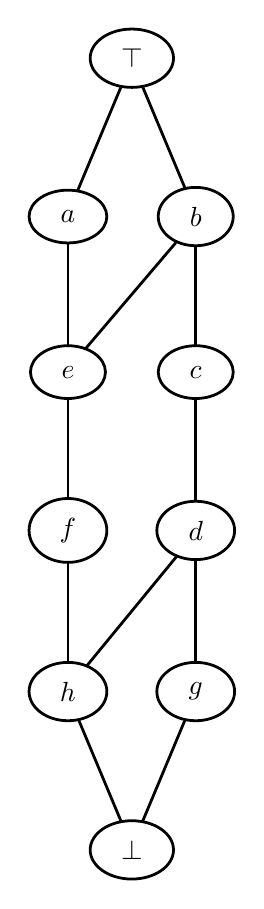
\begin{tikzpicture}[>=latex,line join=bevel]
  \pgfsetlinewidth{1bp}
%%
\pgfsetcolor{black}
  % Edge: \top -- a
  \draw [] (32.994bp,284.92bp) .. controls (28.618bp,274.46bp) and (21.678bp,257.86bp)  .. (17.509bp,247.89bp);
  % Edge: \top -- b
  \draw [] (41.006bp,284.92bp) .. controls (45.279bp,274.7bp) and (51.997bp,258.64bp)  .. (56.192bp,248.61bp);
  % Edge: a -- e
  \draw [] (14.0bp,228.58bp) .. controls (14.0bp,218.52bp) and (14.0bp,202.25bp)  .. (14.0bp,192.25bp);
  % Edge: b -- c
  \draw [] (60.0bp,227.6bp) .. controls (60.0bp,217.49bp) and (60.0bp,201.95bp)  .. (60.0bp,192.27bp);
  % Edge: b -- e
  \draw [] (52.812bp,229.06bp) .. controls (43.918bp,218.62bp) and (28.908bp,201.0bp)  .. (20.396bp,191.01bp);
  % Edge: c -- d
  \draw [] (60.0bp,172.91bp) .. controls (60.0bp,163.0bp) and (60.0bp,146.74bp)  .. (60.0bp,136.33bp);
  % Edge: d -- g
  \draw [] (60.0bp,114.75bp) .. controls (60.0bp,104.47bp) and (60.0bp,88.379bp)  .. (60.0bp,78.143bp);
  % Edge: d -- h
  \draw [] (53.213bp,116.24bp) .. controls (44.515bp,105.65bp) and (29.526bp,87.401bp)  .. (20.815bp,76.797bp);
  % Edge: e -- f
  \draw [] (14.0bp,172.91bp) .. controls (14.0bp,163.24bp) and (14.0bp,147.53bp)  .. (14.0bp,137.1bp);
  % Edge: f -- h
  \draw [] (14.0bp,113.97bp) .. controls (14.0bp,103.7bp) and (14.0bp,88.221bp)  .. (14.0bp,78.236bp);
  % Edge: g -- \bot
  \draw [] (55.994bp,56.92bp) .. controls (51.772bp,46.825bp) and (45.164bp,31.024bp)  .. (40.96bp,20.97bp);
  % Edge: h -- \bot
  \draw [] (18.006bp,56.92bp) .. controls (22.228bp,46.825bp) and (28.836bp,31.024bp)  .. (33.04bp,20.97bp);
  % Node: \top
\begin{scope}
  \definecolor{strokecol}{rgb}{0.0,0.0,0.0};
  \pgfsetstrokecolor{strokecol}
  \draw (37.0bp,295.5bp) ellipse (15.0bp and 10.5bp);
  \draw (37.0bp,295.5bp) node {$\top$};
\end{scope}
  % Node: a
\begin{scope}
  \definecolor{strokecol}{rgb}{0.0,0.0,0.0};
  \pgfsetstrokecolor{strokecol}
  \draw (14.0bp,238.5bp) ellipse (14.0bp and 9.5bp);
  \draw (14.0bp,238.5bp) node {$a$};
\end{scope}
  % Node: b
\begin{scope}
  \definecolor{strokecol}{rgb}{0.0,0.0,0.0};
  \pgfsetstrokecolor{strokecol}
  \draw (60.0bp,238.5bp) ellipse (13.5bp and 10.5bp);
  \draw (60.0bp,238.5bp) node {$b$};
\end{scope}
  % Node: e
\begin{scope}
  \definecolor{strokecol}{rgb}{0.0,0.0,0.0};
  \pgfsetstrokecolor{strokecol}
  \draw (14.0bp,182.5bp) ellipse (13.5bp and 9.5bp);
  \draw (14.0bp,182.5bp) node {$e$};
\end{scope}
  % Node: c
\begin{scope}
  \definecolor{strokecol}{rgb}{0.0,0.0,0.0};
  \pgfsetstrokecolor{strokecol}
  \draw (60.0bp,182.5bp) ellipse (13.5bp and 9.5bp);
  \draw (60.0bp,182.5bp) node {$c$};
\end{scope}
  % Node: d
\begin{scope}
  \definecolor{strokecol}{rgb}{0.0,0.0,0.0};
  \pgfsetstrokecolor{strokecol}
  \draw (60.0bp,125.5bp) ellipse (14.0bp and 10.5bp);
  \draw (60.0bp,125.5bp) node {$d$};
\end{scope}
  % Node: g
\begin{scope}
  \definecolor{strokecol}{rgb}{0.0,0.0,0.0};
  \pgfsetstrokecolor{strokecol}
  \draw (60.0bp,67.5bp) ellipse (14.0bp and 10.5bp);
  \draw (60.0bp,67.5bp) node {$g$};
\end{scope}
  % Node: h
\begin{scope}
  \definecolor{strokecol}{rgb}{0.0,0.0,0.0};
  \pgfsetstrokecolor{strokecol}
  \draw (14.0bp,67.5bp) ellipse (14.0bp and 10.5bp);
  \draw (14.0bp,67.5bp) node {$h$};
\end{scope}
  % Node: f
\begin{scope}
  \definecolor{strokecol}{rgb}{0.0,0.0,0.0};
  \pgfsetstrokecolor{strokecol}
  \draw (14.0bp,125.5bp) ellipse (14.0bp and 11.5bp);
  \draw (14.0bp,125.5bp) node {$f$};
\end{scope}
  % Node: \bot
\begin{scope}
  \definecolor{strokecol}{rgb}{0.0,0.0,0.0};
  \pgfsetstrokecolor{strokecol}
  \draw (37.0bp,10.5bp) ellipse (15.0bp and 10.5bp);
  \draw (37.0bp,10.5bp) node {$\bot$};
\end{scope}
%
\end{tikzpicture}}
\end{frame}
\begin{frame}
\frametitle{Results}
In a residuated binar (with or without involution), none of the following distributivity laws follows from any combination of others:
\begin{align*}
x\cdot(y\wedge z)= x\cdot y\wedge x\cdot z \\
(x\wedge y)\cdot z= x\cdot z\wedge y\cdot z \\
x\backslash (y\vee z) = x\backslash y\vee x\backslash z \\
(x\vee y)/ z = x/ z\vee y/ z \\
(x\wedge y)\backslash z = x\backslash z\vee y\backslash z \\
x/ (y\wedge z) = x/ y \vee x/ z \\
\end{align*}
\end{frame}
\begin{frame}
\frametitle{Results}
\begin{itemize}
\item all examples in the general case are non-modular
\item for modular case Isabelle fails to find counter-examples of size up to 14 for some assumptions
\item results from Fussner\&Jipsen paper might be generalisable to the modular case
\end{itemize}
\end{frame}
\begin{frame}
\frametitle{Was it easy?}
\begin{itemize}
\item running on three Linux machines, the largest having 180 CPU cores (\textsc{Intel}\textsuperscript{\textregistered} \textsc{Xeon}\textsuperscript{\textregistered} Gold 6254 3.10GHz) and 832 GB of RAM
\item about two weeks of wall-time computations
\item filing a kernel bug report to one of the servers' sellers
\item the largest model is of cardinality 10
\end{itemize}
\end{frame}
\begin{frame}
\frametitle{Conclusions}
\begin{itemize}
\item sometimes using newer software helps solving open problems in mathematics
\item collaboration of mathematicians and computer scientists might be fruitful
\item ITPs are not only for formalizations
\end{itemize}
\end{frame}
\begin{frame}
\frametitle{Thank you for your attention!}
Discussion time!
\end{frame}
\end{document}
